\begin{center}
	\textbf{Đề kiểm tra số 2}
\end{center}
\setcounter{ex}{0}% Reset lại số đếm câu hỏi
\Opensolutionfile{ans}[ans/ansCD2D1-7DKt2]
\begin{ex}%[DỰ án LTĐH-Nguyễn Chiến Thắng]%[2D1B1-1]
	Hàm số nào sau đây nghịch biến trên từng khoảng xác định?
	\choice
	{$y=x^4-x^2$}
	{$y=-x^3+3x^2$}
	{$y=2x-\sin x$}
	{\True $y=\dfrac{x-1}{x-2}$}
	\loigiai{
		* Tập xác định $\mathscr{D}=\mathbb{R}\setminus\{2\}$.\\
		* Ta có $y’=\dfrac{-1}{(x-2)^2}<0$, $\forall x\neq 2$ suy ra hàm số nghịch biến trên từng khoảng xác định của hàm số.}
\end{ex}
\begin{ex}%[DỰ án LTĐH-Nguyễn Chiến Thắng]%[2D1B1-2]
	\immini{	Cho hàm số $y=f(x)$ có bảng biến thiên như sau. Tìm giá trị cực đại  $y_{CĐ}$ và giá trị cực tiểu $y_{CT}$ của hàm số đã cho. 
		\choice
		{$y_{CĐ}=4$ và $y_{CT}=-1$}
		{$y_{CĐ}=1$ và $y_{CT}=0$}
		{$y_{CĐ}=-1$ và $y_{CT}=1$}
		{\True $y_{CĐ}=-4$ và $y_{CT}=0$}}{	
\begin{tikzpicture}[>=stealth]
		\tkzTabInit[nocadre=false,lgt=1,espcl=2,deltacl=0.5]{$x$/.7 ,$y'$/.7,$y$/2}
		{$-\infty$ , $-1$ , $1$ , $+\infty$}
		\tkzTabLine{ , + , $0$ , - , $0$ , + , }
		\tkzTabVar{-/$-\infty$ , +/$4$ , -/$0$ , +/$+\infty$}
		\end{tikzpicture}}
\end{ex}
\begin{ex}%[DỰ án LTĐH-Nguyễn Chiến Thắng]%[2D1B4-1]
	Tìm số tiệm cận của đồ thị hàm số $y=\dfrac{3x-4}{x-1}$. 
	\choice
	{\True $2$}
	{$3$}
	{$1$}
	{$0$}
	\loigiai{
		Ta có tập xác định: $\mathscr{D}=\mathbb{R}\setminus\{1\}$.\\
		Do $\lim\limits_{x\to\pm\infty} y=3$ và $\lim\limits_{x\to 1^+} y=-\infty$, $\lim\limits_{x\to 1^-} y=+\infty$ nên đồ thị hàm số có hai đường tiệm cận.}
\end{ex}
\begin{ex}%[DỰ án LTĐH-Nguyễn Chiến Thắng]%[2D1B1-2]
	\immini{	Cho hàm số $y=f(x)$ liên tục trên $\mathbb{R}$ và có bảng biến thiên như hình dưới đây. Khẳng định nào sau đây là sai?
	}{	
\begin{tikzpicture}[>=stealth]
		\tkzTabInit[nocadre=false,lgt=1,espcl=2,deltacl=0.5]{$x$/.7 ,$y'$/.7,$y$/2}
		{$-\infty$ , $-1$ , $1$ , $+\infty$}
		\tkzTabLine{ , - , $0$ , + , $0$ , - , }
		\tkzTabVar{+/$+\infty$ , -/$-1$ , +/$3$ , -/$-\infty$}
		\end{tikzpicture}}
	\choice
	{Hàm số nghịch biến trên khoảng $(-\infty;-1)$}
	{Hàm số đồng biến trên khoảng $(-1;1)$}
	{Hàm số nghịch biến trên khoảng $(1;+\infty)$}
	{\True Hàm số đồng biến trên khoảng $(-1;3)$}
	\loigiai{
		Từ bảng biến thiên ta thấy kết luận hàm số đồng biến trên khoảng $(-1;3)$ là kết luận SAI.}
\end{ex}
\begin{ex}%[DỰ án LTĐH-Nguyễn Chiến Thắng]%[2D1B3-1]
	Tìm giá trị lớn nhất của hàm số $f(x)=\dfrac{x}{x+2}$ trên đoạn $[1;4]$. 
	\choice
	{$\max\limits_{[1;4]} f(x)=\dfrac{1}{3}$}
	{\True $\max\limits_{[1;4]} f(x)=\dfrac{2}{3}$}
	{$\max\limits_{[1;4]} f(x)=1$}
	{Không tồn tại}
	\loigiai{
		Hàm số xác định $[1;4]$.\\
		Có $f’(x)=\dfrac{2}{(x+2)^2}>0,\forall x\in[1; 4]$ nên hàm số đồng biến trên $[1;4]$.\\
		Do đó $\max\limits_{[1;4]} f(x)=f(4)=\dfrac{4}{4+2} =\dfrac{2}{3}$.}
\end{ex}
\begin{ex}%[DỰ án LTĐH-Nguyễn Chiến Thắng]%[2D1B5-1]
	\immini{	Đường cong trong hình bên là đồ thị một hàm số được liệt kê ở bốn phương án $A, B, C, D$ dưới đây. Hỏi hàm số đó là hàm số nào?}{	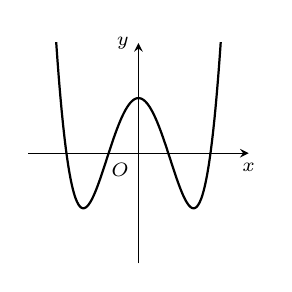
\begin{tikzpicture}[>=stealth,x=1cm,y=1cm,scale=0.7]
		\def\a{1} % Hệ số a phải khác 0
		\def\b{-3}
		\def\c{0}
		\def\d{2}
		\draw[->] (-2,0) -- (2,0)node[below]{\scriptsize $x$};
		\draw[->] (0,-2) -- (0,2) node[left] {\scriptsize $y$};
		\draw (0,0)node[below left]{\scriptsize $O$};
		\clip (-2,-2)rectangle(2,2);
		\draw[thick,samples=150,smooth,domain=-2:2] plot(\x,{2*(\x)^4-(4)*(\x)^2+1});
		\end{tikzpicture}}
	\choice
	{$y=x^3-3x^2+1$}
	{\True $y=2x^4-4x^2+1$}
	{$y=-2x^4+4x^2+1$}
	{$y=-2x^4+4x^2$}
	\loigiai{
		Đồ thị đã cho là đồ thị hàm trùng phương có hệ số $a>0$ và đi qua điểm $(0; 1)\Rightarrow$ loại A, C,D.\\
		Vậy đó là đồ thị hàm số $y=2x^4-4x^2+1$.}
\end{ex}
\begin{ex}%[DỰ án LTĐH-Nguyễn Chiến Thắng]%[2D1B5-8]
	Cho hàm số $y=\dfrac{x-2}{x+1}$. Xét các phát biểu sau đây:\\
	i) Đồ thị hàm số nhận điểm $I(-1;1)$ làm tâm đối xứng.\\
	ii) Hàm số đồng biến trên tập $\mathbb{R}\setminus\{-1\}$.\\
	iii) Giao điểm của đồ thị với trục hoành là điểm $A(0;-2)$.\\
	iv) Tiệm cận đứng là $y=1$ và tiệm cận ngang là $x=-1$.\\
	Trong các phát biểu trên, có bao nhiêu phát biểu đúng
	\choice
	{\True $1$}
	{$3$}
	{$2$}
	{$4$}
	\loigiai{
		Ta có $\lim\limits_{x\to\pm\infty} y =\lim\limits_{x\to\pm\infty}\dfrac{x-2}{x+1}=1$ nên đường thẳng $y=1$ là tiệm cận ngang của đồ thị hàm số.\\
		$\lim\limits_{x\to-1^-} y=\lim\limits_{x\to-1^-}\dfrac{x-2}{x+1}=+\infty$; $\lim\limits_{x\to-1^+} y=\lim\limits_{x\to-1^+}\dfrac{x-2}{x+1}=-\infty$ nên đường thẳng $x=-1$ là tiệm cận đứng của đồ thị hàm số.\\
		Do đó, đồ thị hàm số nhận giao điểm của hai tiệm cận $I(-1;1)$ làm tâm đối xứng. (đúng).\\
		Hàm số đồng biến trên tập $\mathbb{R}\setminus\{-1\}$ là khẳng định sai vì hàm số chỉ đồng biến trên từng khoảng của tập xác định.\\
		Giao điểm của đồ thị với trục hoành là điểm $A(0;-2)$ là khẳng định sai vì điểm $A(0;-2)$ không nằm trên trục hoành.\\
		Tiệm cận đứng là $y=1$ và tiệm cận ngang là $x=-1$ là khẳng định sai. (theo kết quả trên).}
\end{ex}
\begin{ex}%[DỰ án LTĐH-Nguyễn Chiến Thắng]%[2D1K1-2]
	\immini{Hình bên là đồ thị của hàm số $y=f’(x)$. Hỏi đồ thị hàm số $y=f(x)$ đồng biến trên khoảng nào dưới đây?\\
		\choice
		{\True $(2;+\infty)$}
		{$(1;2)$}
		{$(0;1)$}
		{$(0;1)$ và $(2;+\infty)$}}{	\begin{tikzpicture}[>=stealth,x=1cm,y=1cm,scale=0.4]
		\def\a{1} % Hệ số a phải khác 0
		\def\b{-3}
		\def\c{0}
		\def\d{2}
		\draw[->] (-5,0) -- (5,0)node[below]{\scriptsize $x$};
		\draw[->] (0,-5) -- (0,5) node[left] {\scriptsize $y$};
		\draw (0,0)node[below left]{\scriptsize $O$};
		\clip (-5,-5)rectangle(5,5);
		\draw[thick,samples=150,smooth,domain=-5:5] plot(\x,{(\x)^3-(4)*(\x)^2+(5)*\x-2});
		\end{tikzpicture}}
	\loigiai{
		Dựa vào đồ thị $f’(x)$ ta có $f’(x)>0$ khi $x\in(2;+\infty)\Rightarrow$ hàm số $f(x)$ đồng biến trên khoảng $(2;+\infty)$.}
\end{ex}
\begin{ex}%[DỰ án LTĐH-Nguyễn Chiến Thắng]%[2D1K5-4]
	\immini{Cho hàm số $y=f(x)$ xác định trên $\mathbb{R}\setminus\{-1\}$, liên tục trên mỗi khoảng xác định và có bảng biến thiên như hình sau.	Tìm tập hợp tất cả các giá trị của tham số thực $m$ sao cho phương trình $f(x)=m$ có đúng ba nghiệm thực phân biệt
		\choice
		{\True $(-4;2)$}
		{$[-4;2)$}
		{$(-4;2]$}
		{$(-\infty;2]$}}{	
\begin{tikzpicture}[>=stealth]
		\tkzTabInit[nocadre=false,lgt=1,espcl=2,deltacl=0.5]{$x$/.7 ,$y'$/.7,$y$/2}
		{$-\infty$ , $-1$ ,$3$, $+\infty$}
		\tkzTabLine{ , + , d , - , z , + , }
		\tkzTabVar{-/$-\infty$ ,+D+/$2$/$+\infty$, -/$-4$,+/$+\infty$}
		\end{tikzpicture}}
	\loigiai{
		Số nghiệm phương trình $f(x)=m$ là số giao điểm của hai đường $y=f(x)$ và $y=m$: là đường thẳng song song với trục $Ox$ cắt $Oy$ tại điểm có tung độ $m$.\\
		Phương trình có $3$ nghiệm thực phân biệt khi đường thẳng $y=m$ cắt đồ thị $y=f(x)$ tại ba điểm phân biệt.\\
		Dựa vào bảng biến thiên có $m\in(-4;2)$.}
\end{ex}
\begin{ex}%[DỰ án LTĐH-Nguyễn Chiến Thắng]%[2D1K3-1]
	Tích của giá trị nhỏ nhất và giá trị lớn nhất của hàm số $f(x)=x+\dfrac{4}{x}$ trên đoạn $[1; 3]$ bằng 
	\choice
	{$\dfrac{52}{3}$}
	{\True $20$}
	{$6$}
	{$\dfrac{65}{3}$}
	\loigiai{
		Tập xác định: $\mathscr{D}=\mathbb{R}\setminus\{0\}$.\\
		$y’=1-\dfrac{4}{x^2}=\dfrac{x^2-4}{x^2}; y’=0\Leftrightarrow x^2-4=0\Leftrightarrow\hoac{&x=2\in[1; 3]\\&x=-2\notin[1; 3].}$ \\
		Ta có: $f(1)=5; f(2)=4; f(3)=\dfrac{13}{3}$.\\
		Vậy $\max\limits_{[1;3]} y=5;\min\limits_{[1;3]} y=4\Rightarrow\max\limits_{[1;3]} y\cdot\min\limits_{[1;3]} y=20$.}
\end{ex}
\begin{ex}%[DỰ án LTĐH-Nguyễn Chiến Thắng]%[2D1K5-6]
	Phương trình tiếp tuyến của đồ thị hàm số $y=x^2-x-2$ tại điểm có hoành độ $x=1$ là
	\choice
	{$2x-y=0$}
	{$2x-y-4=0$}
	{$x-y-1=0$}
	{\True $x-y-3=0$}
	\loigiai{
		Gọi $M$ là tiếp điểm của tiếp tuyến và đồ thị hàm số. Theo giả thiết: $M(1;-2)$.\\
		Gọi $k$ là hệ số góc của tiếp tuyến với đồ thị hàm số tại $M$.\\
		Ta có $y’=2x-1$, $k=y’(1)=1$.\\
		Phương trình tiếp tuyến cần tìm là $y=1(x-1)-2\Leftrightarrow x-y-3=0$.}
\end{ex}
\begin{ex}%[DỰ án LTĐH-Nguyễn Chiến Thắng]%[2D1K2-4]
	Đồ thị hàm số $y=ax^3+bx^2+cx+d$ có hai điểm cực trị $A(1;-7), B(2;-8)$. Tính $y(-1)$?
	\choice
	{$y(-1)=7$}
	{$y(-1)=11$}
	{$y(-1)=-11$}
	{\True $y(-1)=-35$}
	\loigiai{
		Ta có: $y’=3ax^2+2bx+c$.\\
		Theo bài cho ta có: $\heva{&3a+2b+c=0\\&12a+4b+c=0\\&a+b+c+d=-7\\&8a+4b+2c+d=-8}\Leftrightarrow\heva{&3a+2b+c=0\\&12a+4b+c=0\\&7a+3b+c=-1\\&d=-7-a-b-c}\Leftrightarrow\heva{&a=2\\&b=-9\\&c=12\\&d=-12.}$ \\
		Suy ra: $y=2x^3-9x^2+12x-12$. Do đó, $y(-1)=-35$.}
\end{ex}
\begin{ex}%[DỰ án LTĐH-Nguyễn Chiến Thắng]%[2D1K2-4]
	Có bao nhiêu giá trị nguyên của $m$ để hàm số $f(x)=2x^3-6x^2-m+1$ có các giá trị cực trị trái dấu?
	\choice
	{$2$}
	{$9$}
	{$3$}
	{\True $7$}
	\loigiai{
		TXĐ: $\mathscr{D}=\mathbb{R}$.\\
		$f’(x)=6x^2-12x=6x(x-2)$.\\
		$f’(x)=0\Leftrightarrow\hoac{&x_1=0\\&x_2=2}$. Khi đó: $y_1=y(0)=1-m$ và $y_1=y(2)=-7-m$.\\
		Để hai giá trị cực trị trái dấu cần có: $y_1\cdot y_2<0\Leftrightarrow(1-m)(-m-7)<0\Leftrightarrow-7<m<1$.\\
		Mà $m\in\mathbb{Z}\Rightarrow m\in\left\{-6;-5;-4;-3;-2;-1;0\right\}$.}
\end{ex}
\begin{ex}%[DỰ án LTĐH-Nguyễn Chiến Thắng]%[2D1K3-1]
	Gọi $M$ và $m$ lần lượt là giá trị lớn nhất và giá trị nhỏ nhất của hàm số $y=\dfrac{\sqrt{x^2-1}}{x-2}$ trên tập $\mathscr{D}=(-\infty;-1]\cup\left[1;\dfrac{3}{2}\right]$. Tính giá trị $T$ của $m.M$. 
	\choice
	{$T=\dfrac{1}{9}$}
	{$T=\dfrac{3}{2}$}
	{\True $T=0$}
	{$T=-\dfrac{3}{2}$}
	\loigiai{
		$y=\dfrac{\sqrt{x^2-1}}{x-2}$. Tập xác định $(-\infty;-1]\cup[1;+\infty)\setminus\{2\}$.\\
		$\begin{aligned}&y’=\dfrac{\dfrac{x(x-2)}{\sqrt{x^2-1}}-\sqrt{x^2-1}}{(x-2)^2}=\dfrac{-2x+1}{\sqrt{x^2-1}(x-2)^2}\\&y’=0\Leftrightarrow x=\dfrac{1}{2}\end{aligned}$ 
		
\begin{tikzpicture}[>=stealth]
		\tkzTabInit[nocadre=false,lgt=1,espcl=2,deltacl=0.5]{$x$/.7 ,$y'$/.7,$y$/2}
		{$-\infty$, $-1$, $\dfrac{1}{2}$ , $1$, $\dfrac{3}{2}$}
		\tkzTabLine{, +, , h, , -,  }
		\tkzTabVar{-/$-1$ , +H/$0$ , ,+/$-1$,-/$-\sqrt{5}$}
		\end{tikzpicture}
		
		Từ bảng biến thiên suy ra $M=0; m=-\sqrt{5}$.\\
		Vậy $M.m=0$.}
\end{ex}
\begin{ex}%[DỰ án LTĐH-Nguyễn Chiến Thắng]%[2D1B4-1]
	Số tiệm cận ngang của đồ thị hàm số $y=2x-1+\sqrt{4x^2-4}$ là
	\choice
	{$2$}
	{\True $1$}
	{$0$}
	{$3$}
	\loigiai{
		Ta có $\lim\limits_{x\to+\infty} y=\lim\limits_{x\to+\infty}\left(2x-1+\sqrt{4x^2-4}\right)=+\infty$;\\
		$\begin{aligned}&\lim\limits_{x\to-\infty} y=\lim\limits_{x\to-\infty}\left(2x-1+\sqrt{4x^2-4}\right)=\lim\limits_{x\to-\infty}\dfrac{(2x-1)^2-\left(4x^2-4\right)}{2x-1-\sqrt{4x^2-4}}\\&=\lim\limits_{x\to-\infty}\dfrac{-4x+5}{2x-1-\sqrt{4x^2-4}}=\dfrac{-4}{2+2}=-1\cdot\end{aligned}$.\\
		Nên đồ thị hàm số chỉ có một tiệm cận ngang là đường thẳng $y=-1$.}
\end{ex}
\begin{ex}%[DỰ án LTĐH-Nguyễn Chiến Thắng]%[2D1K1-3]
	Tìm giá trị lớn nhất của tham số $m$ để hàm số $y=\dfrac{1}{3}x^3-mx^2+(8-2m)x+m+3$ đồng biến trên $\mathbb{R}$. 
	\choice
	{\True $m=2$}
	{$m=-2$}
	{$m=4$}
	{$m=-4$}
	\loigiai{
		TXĐ: $\mathscr{D}=\mathbb{R}$.\\
		Ta có $y’=x^2-2mx+(8-2m)$. Để hàm số đồng biến trên $\mathbb{R}$ thì $y’\geq 0,\forall x\in\mathbb{R}$.\\
		(Dấu chỉ xảy ra tại hữu hạn điểm trên $\mathbb{R}$).\\
		ĐK: $\Delta\leq 0\Rightarrow m^2+2m-8\leq 0\Leftrightarrow-4\leq m\leq 2$.\\
		Vậy giá trị lớn nhất của $m$ để hàm số đồng biến trên $\mathbb{R}$ là $m=2$.}
\end{ex}
\begin{ex}%[DỰ án LTĐH-Nguyễn Chiến Thắng]%[2D1K1-3]
	Cho hàm số $y=ax^3+bx^2+cx+d$. Hỏi hàm số luôn đồng biến trên $\mathbb{R}$ khi nào?
	\choice
	{$\hoac{&a=b=0, c>0\\&a>0; b^2-3ac\geq 0}$}
	{$\hoac{&a=b=c=0\\&a<0; b^2-3ac<0}$}
	{\True $\hoac{&a=b=0, c>0\\&a>0; b^2-3ac\leq 0}$}
	{$\hoac{&a=b=0, c>0\\&a<0; b^2-3ac\leq 0}$}
	\loigiai{
		Hàm số luôn đồng biến trên $\mathbb{R}$ khi $y’=3ax^2+2bx+c\geq 0,\forall x\in\mathbb{R}$.\\
		Trường hợp 1: $a=b=0, c>0$.\\
		Trường hợp 1: $a\neq 0$, giải $\Delta’=b^2-3ac$.\\
		Hàm số luôn đồng biến trên $\mathbb{R}\Leftrightarrow y’\geq 0,\forall x\in\mathbb{R}\Leftrightarrow\heva{&a>0\\&\Delta’\leq 0}\Leftrightarrow\heva{&a>0\\&b^2-3ac\leq 0}$.}
\end{ex}
\begin{ex}%[DỰ án LTĐH-Nguyễn Chiến Thắng]%[2D1K4-1]
	Số đường tiệm cận đứng của đồ thị hàm số $y=\dfrac{\left(x^2-3x+2\right)\sin x}{x^3-4x}$ là 
	\choice
	{\True $1$}
	{$2$}
	{$3$}
	{$4$}
	\loigiai{
		TXĐ: $\mathscr{D}=\mathbb{R}\setminus\{0;-2;2\}$.\\
		$\lim\limits_{x\to 0} y=\lim\limits_{x\to 0}\left[\left(\dfrac{x^2-3x+2}{x^2-4}\right)\left(\dfrac{\sin x}{x}\right)\right]=\dfrac{0^2-3\cdot 0+2}{0^2-4}\cdot 1=-\dfrac{1}{2}$.\\
		$\lim\limits_{x\to-2^{\pm}} y=\lim\limits_{x\to-2^{\pm}}\left[\dfrac{\left(x^2-3x+2\right)\sin x}{x\left(x^2-4\right)}\right]=\lim\limits_{x\to-2^{\pm}}\left[\dfrac{(x-1)(x-2)\sin x}{x(x-2)}\cdot\dfrac{1}{(x+2)}\right]$.\\
		$=\lim\limits_{x\to-2^{\pm}}\left[\dfrac{(x-1)\sin x}{x}\cdot\dfrac{1}{(x+2)}\right]$.\\
		o Vì $\lim\limits_{x\to-2^+}\left[\dfrac{(x-1)\sin x}{x}\right]=-\dfrac{3\sin 2}{2}<0$ và $\lim\limits_{x\to-2^+}\dfrac{1}{(x+2)}=+\infty$ nên $\lim\limits_{x\to-2^+} y=-\infty$.\\
		o Vì $\lim\limits_{x\to-2^-}\left[\dfrac{(x-1)\sin x}{x}\right]=-\dfrac{3\sin 2}{2}<0$ và $\lim\limits_{x\to-2^-}\dfrac{1}{(x+2)}=-\infty$ nên $\lim\limits_{x\to-2^-} y=+\infty$.\\
		Vậy đường thẳng $x=-2$ là tiệm cận đứng của đồ thị hàm số.\\
		$\lim\limits_{x\to 2} y=\lim\limits_{x\to 2}\dfrac{(x-1)\sin x}{x(x+2)}=\dfrac{\sin 2}{6}$.\\
		Vậy ĐTHS có $1$ đường tiệm cận đứng.}
\end{ex}
\begin{ex}%[DỰ án LTĐH-Nguyễn Chiến Thắng]%[2D1K1-3]
	Tìm tập hợp $S$ tất cả các giá trị của tham số thực $m$ để hàm số $y=\dfrac{1}{3}x^3-(m+1)x^2+\left(m^2+2m\right)x-3$ nghịch biến trên khoảng $(-1;1)$. 
	\choice
	{$S=[-1;0]$}
	{$S=\emptyset$}
	{\True $S=\{-1\}$}
	{$S=[0;1]$}
	\loigiai{
		Ta có $y’=x^2-2(m+1)x+\left(m^2+2m\right)$.\\
		Xét $y’=0\Leftrightarrow x^2-2(m+1)x+\left(m^2+2m\right)=0\Leftrightarrow\hoac{&x=m\\&x=m+2}\forall m$.\\
		Hàm số luôn nghịch biến trong khoảng $(m; m+2)\forall m$.\\
		Để hàm số nghịch biến trên khoảng $(-1;1)$ thì $(-1;1)\subset(m; m+2)$.\\
		Nghĩa là $m\leq-1<1\leq m+2\Leftrightarrow\heva{&m\leq-1\\&-1<1\\&1\leq m+2}\Leftrightarrow m=-1$.}
\end{ex}
\begin{ex}%[DỰ án LTĐH-Nguyễn Chiến Thắng]%[2D1K5-4]
	Có bao nhiêu giá trị nguyên của tham số $m$ để đồ thị của hàm số $y=x^3+(m+2)x^2+\left(m^2-m-3\right)x-m^2$ cắt trục hoành tại ba điểm phân biệt?
	\choice
	{$4$}
	{\True $3$}
	{$1$}
	{$2$}
	\loigiai{
		Phương trình hoành độ giao điểm của đồ thị và trục hoành:\\
		$x^3+(m+2)x^2+\left(m^2-m-3\right)x-m^2=0 (1)$ \\
		$ \Leftrightarrow(x-1)\left(x^2+(m+3)x+m^2\right)=0\Leftrightarrow\hoac{&x=1\\&x^2+(m+3)x+m^2=0 (2).} $ \\
		Đồ thị cắt $Ox$ tại 3 điểm phân biệt $\Leftrightarrow$ pt (1) có 3 nghiệm phân biệt\\
		$ \Leftrightarrow $ pt (2) có 2 nghiệm phân biệt khác 1.
		$\Leftrightarrow\heva{&a\neq 0\\&\Delta>0\\&1+m+3+m^2\neq 0}\Leftrightarrow-3m^2+6m+9>0\Leftrightarrow-1<m<3$.\\
		Các giá trị nguyên của $m$ thỏa yêu cầu bài toán là $0,1,2$.}
\end{ex}
\begin{ex}%[DỰ án LTĐH-Nguyễn Chiến Thắng]%[2D1K2-4]
	Cho hàm số $y=(m+1)x^4-(m-1)x^2+1$. Số các giá trị nguyên của $m$ để hàm số có một điểm cực đại mà không có điểm cực tiểu là 
	\choice
	{$1$}
	{\True $0$}
	{$3$}
	{$2$}
	\loigiai{
		Trường hợp $m=-1$, suy ra $y=2x^2+1\Rightarrow$ Hàm số có điểm cực tiểu mà không có điểm cực đại nên loại $m=-1$.\\
		Trường hợp $m\neq-1$.\\
		Ta có: $y’=4(m+1)x^3-2(m-1)x =2x\left[2(m+1)x^2-(m-1)\right]$.\\
		Xét $y’=0\Leftrightarrow\hoac{&x=0\\&g(x)=2(m+1)x^2-(m-1)=0(*)}$.}
\end{ex}
\begin{ex}%[DỰ án LTĐH-Nguyễn Chiến Thắng]%[2D1K4-3]
	Tìm tọa độ điểm $M$ có hoành độ dương thuộc đồ thị $(C)$ của hàm số $y=\dfrac{x+2}{x-2}$ sao cho tổng khoảng cách từ $M$ đến hai đường tiệm cận của đồ thị $(C)$ đạt giá trị nhỏ nhất. 
	\choice
	{$M(1;-3)$}
	{$M(3;5)$}
	{$M(0;-1)$}
	{\True $M(4;3)$}
	\loigiai{
		Tiệm cận đứng: $d_1\colon x-2=0$ và tiệm cận đứng: $d_2\colon y-1=0$.\\
		Với $M\in(C)\colon y=\dfrac{x+2}{x-2}\Rightarrow M\left(x_0;\dfrac{x_0+2}{x_0-2}\right)$ với $x_0>0$, $x_0\neq 2$.\\
		Ta có: $\mathrm{d}\left(M;(d_1)\right)+\mathrm{d}\left(M;(d_2)\right)$.\\
		$=|x_0-2|+\left|\dfrac{x_0+2}{x_0-2}-1\right|=|x_0-2|+\left|\dfrac{4}{x_0-2}\right|\geq 2\sqrt{|x_0-2|\cdot\left|\dfrac{4}{x_0-2}\right|}=4$.\\
		(Áp dụng BĐT Cauchy cho 2 số dương $|x_0-2|$, $\left|\dfrac{4}{x_0-2}\right|$).\\
		Dấu xảy ra khi\\
		$\heva{&|x_0-2|=\left|\dfrac{4}{x_0-2}\right|\\&x_0>0,x_0\neq 2}\Leftrightarrow\heva{&(x_0-2)^2=4\\&x_0>0,x_0\neq 2}\Leftrightarrow\heva{&\hoac{&x_0=4\\&x_0=0}\\&x_0>0,x_0\neq 2}\Leftrightarrow x_0=4\Rightarrow M(4;3)$.\\
		Vì hàm trùng phương luôn đạt cực trị tại điểm $x=0$ nên để hàm số có một điểm cực đại mà không có điểm cực tiểu thì $\heva{&m+1<0\\&-m+1\leq 0}\Leftrightarrow\heva{&m <-1\\&m\geq 1}$, suy ra không tồn tại $m$ thỏa yêu cầu bài toán.}
\end{ex}
\begin{ex}%[DỰ án LTĐH-Nguyễn Chiến Thắng]%[2D1K5-4]
	Cho hàm số $y=x^3-3x^2+(m+1)x+1$ có đồ thị $(C_m)$, với $m$ là tham số. Tìm tất cả các giá trị thực của tham số $m$ để đường thẳng $d\colon y=x+1$ cắt đồ thị $(C_m)$ tại ba điểm phân biệt $\mathrm{P}(0; 1)$, $M$, $N$ sao cho tam giác $OMN$ vuông tại $O$ với $O$ là gốc tọa độ. 
	\choice
	{\True $m=-2$}
	{$m=-6$}
	{$m=-3$}
	{$m=-\dfrac{7}{2}$}
	\loigiai{
		Hoành độ giao điểm là nghiệm của phương trình.\\
		$\begin{aligned}&x^3-3x^2+(m+1)x+1=x+1\Leftrightarrow x^3-3x^2+mx=0(*)\\&\Leftrightarrow x\left(x^2-3x+m\right)=0\Leftrightarrow\hoac{&x=0\\&x^2-3x+m=0\cdot}.\end{aligned}$ \\
		Phương trình $(*)$ có ba nghiệm phân biệt khi và chỉ khi phương trình $x^2-3x+m=0$ có hai nghiệm phân biệt khác $0$ hay.\\
		Gọi $x_1, x_2$ là hai nghiệm phân biệt của phương trình $x^2-3x+m=0$.\\
		Theo Vi-ét $\heva{&x_1+x_2=3\\&x_1x_2=m.}$ \\
		Tọa độ $M(x_1; x_1+1), N(x_2; x_2+1)$. Khi đó tam giác $OMN$ vuông tại $O$ khi và chỉ khi
		.}
\end{ex}
\begin{ex}%[DỰ án LTĐH-Nguyễn Chiến Thắng]%[2D1G3-5]
	Cho $x$, $y$ là các số thực thỏa mãn $x+y=\sqrt{x-1}+\sqrt{2y+2}$. Gọi $M$, $m$ lần lượt là giá trị lớn nhất và nhỏ nhất của $P=x^2+y^2+2(x+1)(y+1)+8\sqrt{4-x-y}$. Tình giá trị $M+m$. 
	\choice
	{$41$}
	{$44$}
	{$42$}
	{\True $43$}
	\loigiai{
		Đk: $x\geq 1;y\geq-1$. Đặt $t=x+y$; $t\geq 0$.\\
		Có $\sqrt{x-1}+\sqrt{2y+2}=\sqrt{x-1}+\sqrt{2}\cdot\sqrt{y+1}\leq\sqrt{3(x+y)}\Rightarrow x+y\leq\sqrt{3(x+y)}$.\\
		Vậy $t\leq\sqrt{3t}\Leftrightarrow t^2-3t\leq 0\Leftrightarrow 0\leq t\leq 3$.\\
		$P=(x+y)^2+2(x+y)+2+8\sqrt{4-(x+y)}$ nên $P=t^2+2t+2+8\sqrt{4-t}$.\\
		$P’=2t+2-\dfrac{4}{\sqrt{4-t}}$.\\
		$P’=0\Leftrightarrow(2t+2)\sqrt{4-t}=4\Leftrightarrow\hoac{&t=0\\&t=1\pm 2\sqrt{2}\notin[0;3].}$ \\
		$\mathrm{P}(0)=18;\mathrm{P}(3)=25$.\\
		Suy ra $M=25;m=18\Rightarrow M+m=43$.}
%<MyLT>
\end{ex}
\begin{ex}%[DỰ án LTĐH-Nguyễn Chiến Thắng]%[2D1G1-4]
	\immini{Cho hàm số $y=f(x)$ có đồ thị như hình vẽ bên. Phương trình $\left|f(x-2)-2\right|=\pi$ có bao nhiêu nghiệm thực phân biệt?
		\choice
		{$4$}
		{\True $2$}
		{$6$}
		{$3$}
	}{	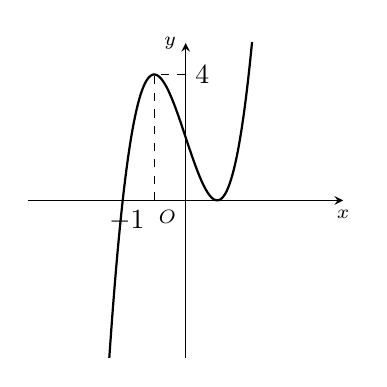
\begin{tikzpicture}[>=stealth,x=1cm,y=1cm,scale=0.4]
		\def\a{1} % Hệ số a phải khác 0
		\def\b{-3}
		\def\c{0}
		\def\d{2}
		\draw[->] (-5,0) -- (5,0)node[below]{\scriptsize $x$};
		\draw[->] (0,-5) -- (0,5) node[left] {\scriptsize $y$};
		\draw (0,0)node[below left]{\scriptsize $O$};
		\coordinate[label=right:$4$](A) at (0,4); % Vị trí đặt nhãn điểm là dưới trái điểm A
		\coordinate[label=below left:$-1$](B) at (-1,0); % Vị trí đặt nhãn điểm là dưới trái điểm A
		\coordinate (C) at (-1,4);
		\draw[line width=0.4pt,dashed,black] (A)--(C)--(B); % Đoạn thẳng AB
		
		\clip (-5,-5)rectangle(5,5);
		\draw[thick,samples=150,smooth,domain=-5:5] plot(\x,{(\x)^3-(3)*(\x)+(2)});
		\end{tikzpicture}}
	\loigiai{
		+ Tịnh tiến đồ thị $y=f(x)$ theo véc-tơ $\overrightarrow{u}=(2;0)$ ta được đồ thị hàm số $y=f(x-2)$ (hình a).\\
		+ Tịnh tiến đồ thị $y=f(x-2)$ theo véc-tơ $\overrightarrow{v}=(0;-2)$ ta được đồ thị hàm số $y=f(x-2)-2$ (hình b).\\
		+ Vẽ đồ thị hàm số $y=\left|f(x-2)-2\right|$ như hình c.
		\begin{center}
			\begin{tikzpicture}[>=stealth,x=1cm,y=1cm,scale=0.6]
			\def\a{1} % Hệ số a phải khác 0
			\def\b{-3}
			\def\c{0}
			\def\d{2}
			\draw[->] (-3,0) -- (5,0)node[below]{\scriptsize $x$};
			\draw[->] (0,-5) -- (0,5) node[left] {\scriptsize $y$};
			\draw (0,0)node[below left]{\scriptsize $O$};
			\coordinate[label= above right:$4$](A) at (0,4); % Vị trí đặt nhãn điểm là dưới trái điểm A
			\coordinate[label=below left:$-1$](B) at (-1,0); % Vị trí đặt nhãn điểm là dưới trái điểm A
			\coordinate (C) at (-1,4);	\coordinate (D) at (1,4);	\coordinate[label=below left:$1$] (E) at (1,0);
			\draw[line width=0.4pt,dashed,black] (A)--(C)--(B) (C)--(D)--(E); % Đoạn thẳng AB
			
			\clip (-5,-5)rectangle(5,5);
			\draw[dashed,red,samples=150,smooth,domain=-5:5] plot(\x,{(\x)^3-(3)*(\x)+(2)});
			\draw[thick,blue,samples=150,smooth,domain=-5:5] plot(\x,{(\x-2)^3-(3)*(\x-2)+(2)});
			\end{tikzpicture}\quad
			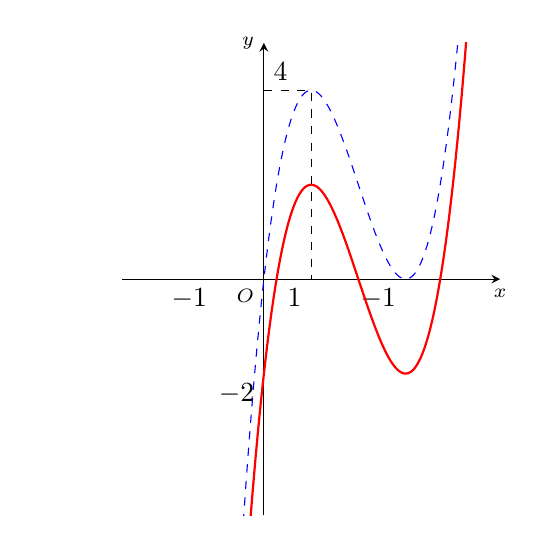
\begin{tikzpicture}[>=stealth,x=1cm,y=1cm,scale=0.6]
			\def\a{1} % Hệ số a phải khác 0
			\def\b{-3}
			\def\c{0}
			\def\d{2}
			\draw[->] (-3,0) -- (5,0)node[below]{\scriptsize $x$};
			\draw[->] (0,-5) -- (0,5) node[left] {\scriptsize $y$};
			\draw (0,0)node[below left]{\scriptsize $O$};
			\coordinate[label=above right:$4$](A) at (0,4); % Vị trí đặt nhãn điểm là dưới trái điểm A
			\coordinate[label=below left:$-1$](B) at (-1,0); % Vị trí đặt nhãn điểm là dưới trái điểm A
			\coordinate[label=below left:$1$](F) at (1,0); % Vị trí đặt nhãn điểm là dưới trái điểm A
			\coordinate[label=below left:$-1$](G) at (3,0); % Vị trí đặt nhãn điểm là dưới trái điểm A
			\coordinate[label=below left:$-2$](H) at (0,-2); % Vị trí đặt nhãn điểm là dưới trái điểm A
			\coordinate (D) at (1,4);	\coordinate (E) at (1,0);
			\draw[line width=0.4pt,dashed,black]  (A)--(D)--(E); % Đoạn thẳng AB			
			\clip (-5,-5)rectangle(5,5);
			\draw[dashed,blue,samples=150,smooth,domain=-5:5] plot(\x,{(\x-2)^3-(3)*(\x-2)+(2)});
			\draw[thick,red,samples=150,smooth,domain=-5:5] plot(\x,{(\x-2)^3-(3)*(\x-2)});
			\end{tikzpicture}\quad
			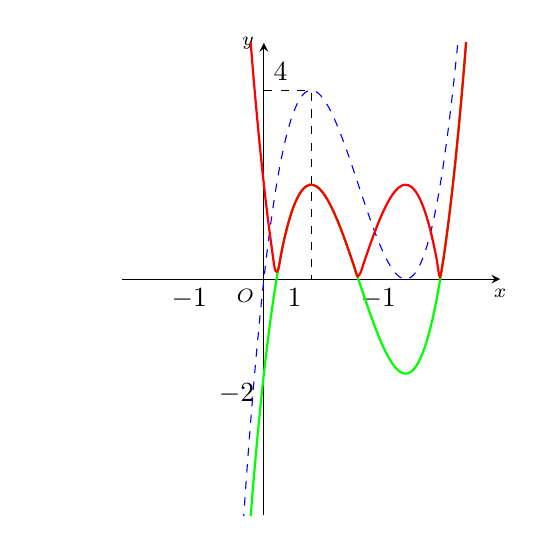
\begin{tikzpicture}[>=stealth,x=1cm,y=1cm,scale=0.6]
			\def\a{1} % Hệ số a phải khác 0
			\def\b{-3}
			\def\c{0}
			\def\d{2}
			\draw[->] (-3,0) -- (5,0)node[below]{\scriptsize $x$};
			\draw[->] (0,-5) -- (0,5) node[left] {\scriptsize $y$};
			\draw (0,0)node[below left]{\scriptsize $O$};
			\coordinate[label=above right:$4$](A) at (0,4); % Vị trí đặt nhãn điểm là dưới trái điểm A
			\coordinate[label=below left:$-1$](B) at (-1,0); % Vị trí đặt nhãn điểm là dưới trái điểm A
			\coordinate[label=below left:$1$](F) at (1,0); % Vị trí đặt nhãn điểm là dưới trái điểm A
			\coordinate[label=below left:$-1$](G) at (3,0); % Vị trí đặt nhãn điểm là dưới trái điểm A
			\coordinate[label=below left:$-2$](H) at (0,-2); % Vị trí đặt nhãn điểm là dưới trái điểm A
			\coordinate (D) at (1,4);	\coordinate (E) at (1,0);
			\draw[line width=0.4pt,dashed,black]  (A)--(D)--(E); % Đoạn thẳng AB		
			\clip (-5,-5)rectangle(5,5);
			\draw[dashed,blue,samples=150,smooth,domain=-5:5] plot(\x,{(\x-2)^3-(3)*(\x-2)+(2)});
			\draw[thick,green,samples=150,smooth,domain=-5:5] plot(\x,{(\x-2)^3-(3)*(\x-2)});
			\draw[thick,red,samples=150,smooth,domain=-5:5] plot(\x,{abs((\x-2)^3-(3)*(\x-2))});
			\end{tikzpicture}
		\end{center}		
		Dựa vào đồ thị hàm số $y=\left|f(x-2)-2\right|$ suy ra phương trình $\left|f(x-2)-2\right|=\pi$ có hai nghiệm thực phân biệt.}
%<MyLT>
\end{ex}
\Closesolutionfile{ans}
\DAPAN
\inputansbox{10}{ans/ansCD2D1-7DKt2}

